\documentclass[dvipdfmx, 12pt]{article}
\usepackage{mathpazo}
\usepackage{amsmath,amssymb}
\usepackage{array}
\usepackage[hiresbb]{graphicx}
\usepackage{tikz}
\usepackage{textcomp}
\usepackage{dcolumn}
\usepackage{here}
\usepackage{lscape}
\usepackage[top=25truemm,bottom=30truemm,left=25truemm,right=25truemm]
{geometry}
\begin{document}

\section{Full-Sample at least 200PAs}



\begin{table}[H]
  \small
  \centering
  \begin{tabular}{lcccccc}\hline
    index & type & cutpoint & binsize & bandwidth & $\theta$ & $z$
    \\ \hline \hline
    AVG & rate & .300 & .001 & .019 &  .499 & 7.442*** \\
    & & & & & (0.067) & \\
    OBP & rate & .350 & .001 & .024 &  .139 & 2.854** \\
    & & & & & (0.049) &  \\
    HR & cumulative & 20 & 1 & 5.309 & .259 & 3.465*** \\
    & & & & & (.075)  & \\
    RBI & cumulative & 100 & 4 & 15.423 & .311 & 3.295*** \\
    & & & & & (0.094) & \\
    SB & cumulative & 30 & 1 & 10.000 & .529 & 4.274*** \\
    & & & & & (.124) & \\
    & & 40 & 1 & 11.505 & .481 & 2.764** \\
    & & & & & (.174) & \\
    PA & cumulative & 500 & 1 & 0.003 & .160 & 2.515* \\
    & & & & &(.063) & \\
    H & cumulative & 200 & 1 & 18.922 & .453 & 2.547 * \\
    & & & & & (.178) & \\ \hline \hline
  \end{tabular}
  \footnotesize
  \flushright
      ***: $p<0.1\%$, **: $p<1\%$, *: $p<5\%$.

    Bandwidth is optimized following the method of Mcrary(2007).
  \caption{Test for Manipulation :leastPA $= 200$}
\end{table}

\newpage

\begin{tabular}{cc}
  \begin{minipage}[H]{0.4\textwidth}

    \begin{figure}[H]
      \centering
      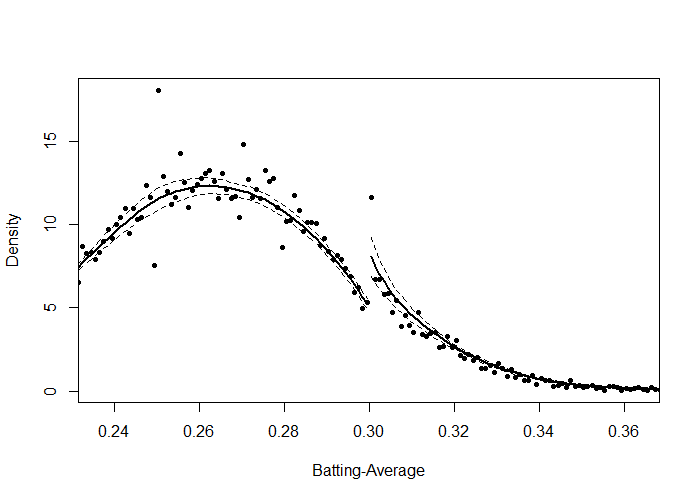
\includegraphics[keepaspectratio, scale = 0.5, angle = 90]
      {graphs/AVG_300.png}
      \caption{AVG (at least 200PA)}
      \label{AVG_300}
    \end{figure}
  \end{minipage} &



  \begin{minipage}[H]{0.4\textwidth}

    \begin{figure}[H]
      \centering
      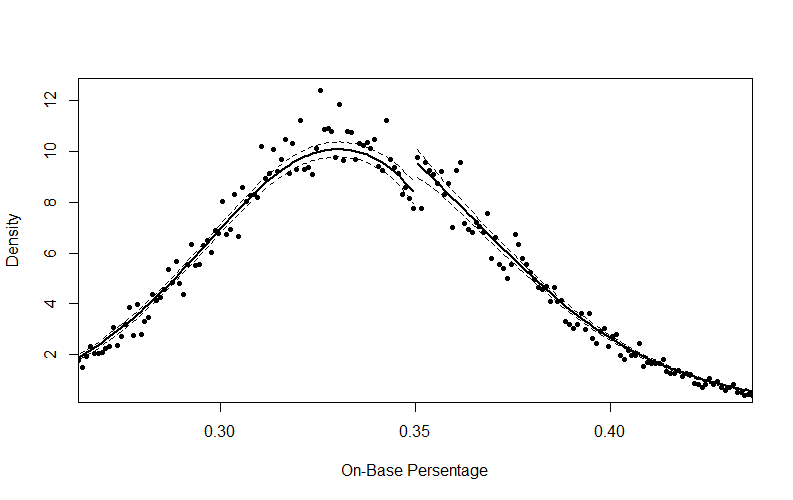
\includegraphics[keepaspectratio, scale = 0.5, angle = 90]
      {graphs/OBP_350.png}
      \caption{OBP (at least 200PA)}
      \label{OBP_350}
      \end{figure}
   \end{minipage} \\
   \begin{minipage}[H]{0.4\textwidth}
    \begin{figure}[H]
      \centering
      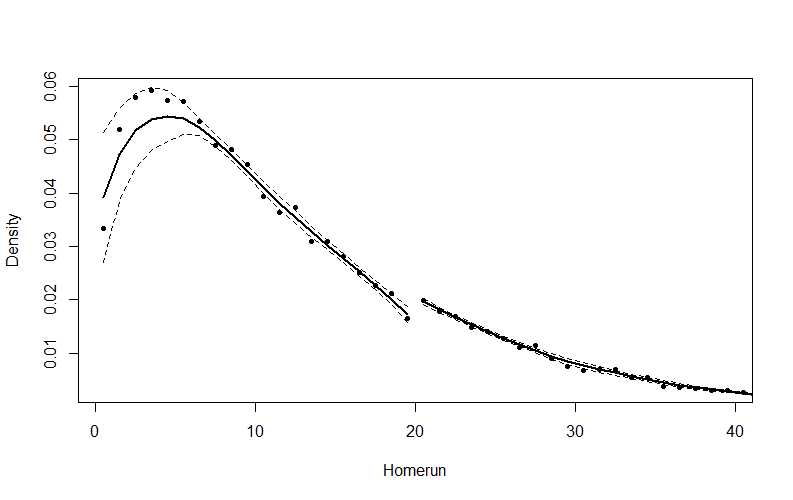
\includegraphics[keepaspectratio, scale = 0.5, angle = 90]
      {graphs/HR_20.png}
      \caption{HR (at least 200PA)}
      \label{HR_20}
    \end{figure}
   \end{minipage}  &

   \begin{minipage}[H]{0.4\textwidth}

    \begin{figure}[H]
      \centering
      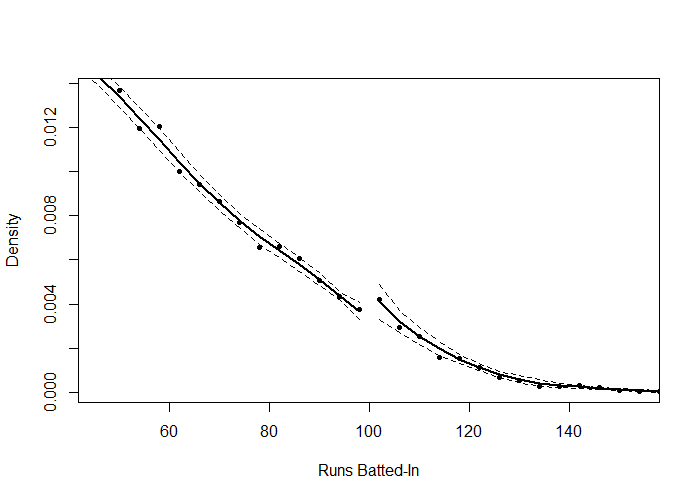
\includegraphics[keepaspectratio, scale = 0.5, angle = 90]
      {graphs/RBI_100.png}
      \caption{RBI (at least 200PA)}
      \label{RBI_100}
    \end{figure}
  \end{minipage}
\end{tabular}

\newpage

\begin{tabular}{cc}
  \begin{minipage}[H]{0.5\textwidth}
    \begin{figure}[H]
      \centering
      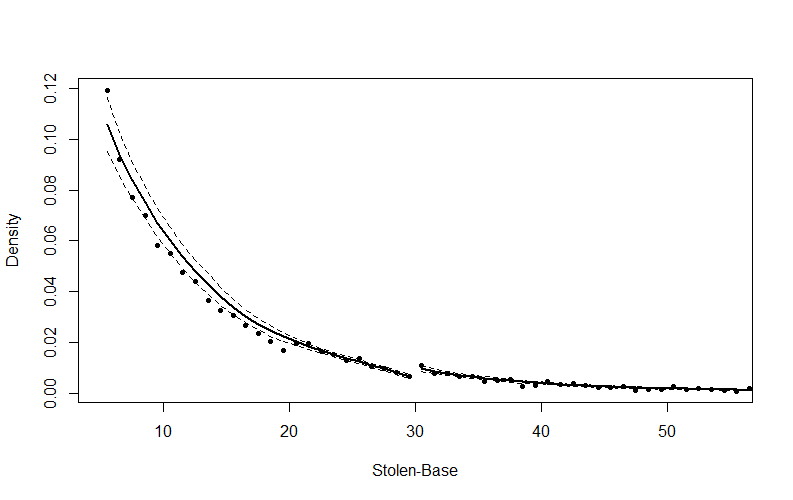
\includegraphics[keepaspectratio, scale = 0.5, angle = 90]
      {graphs/SB_30.png}
      \caption{SB: cutpoint $=30$ (at least 5SB)}
      \label{SB_30}
    \end{figure}

  \end{minipage} &
  \begin{minipage}[H]{0.5\textwidth}
    \begin{figure}[H]
      \centering
      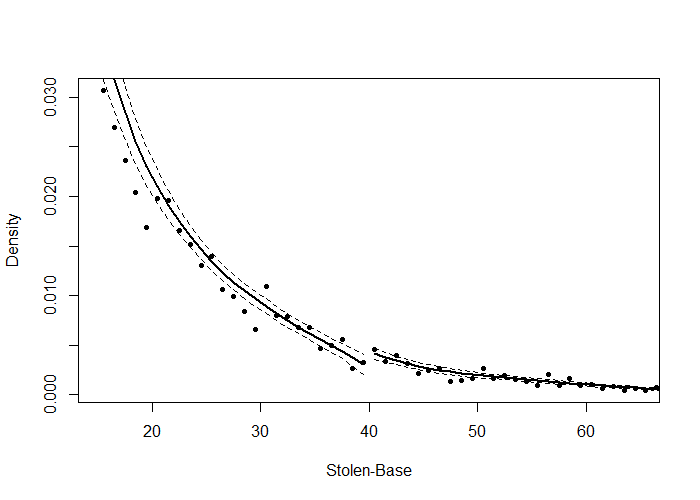
\includegraphics[keepaspectratio, scale = 0.5, angle = 90]
      {graphs/SB_40.png}
      \caption{SB: cutpoint $=40$ (at least 5SB)}
      \label{SB_40}
    \end{figure}

  \end{minipage}\\
  \begin{minipage}[H]{0.5\textwidth}
    \begin{figure}[H]
      \centering
      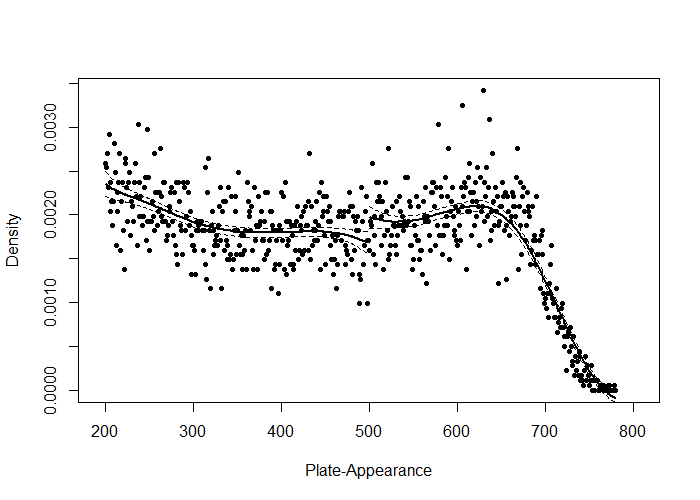
\includegraphics[keepaspectratio, scale = 0.5, angle = 90]
      {graphs/PA_500.png}
      \caption{PA (at least 200PA)}
      \label{PA_500}
    \end{figure}

  \end{minipage}&
  \begin{minipage}[H]{0.5\textwidth}
    \begin{figure}[H]
      \centering
      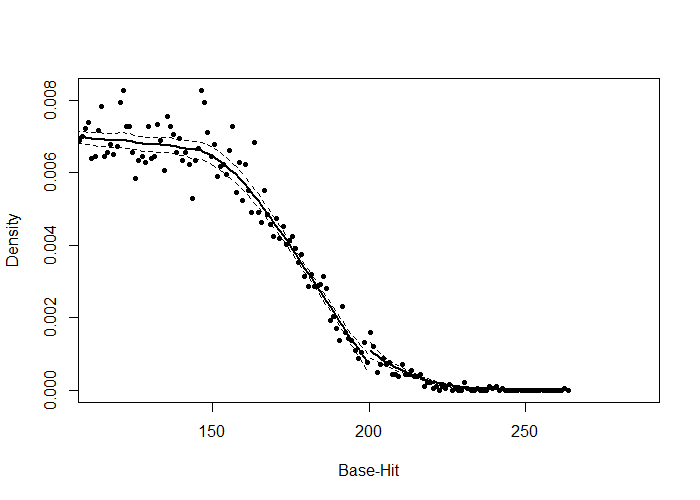
\includegraphics[keepaspectratio, scale = 0.5, angle = 90]
      {graphs/H_200.png}
      \caption{H (at least 200PA)}
      \label{H_200}
    \end{figure}

  \end{minipage}
\end{tabular}

\newpage

\section{Monetary Incentive}

\begin{landscape}
  \begin{table}
    
% Table created by stargazer v.5.2.2 by Marek Hlavac, Harvard University. E-mail: hlavac at fas.harvard.edu
% Date and time: ��, 10 30, 2018 - 14:13:47
% Requires LaTeX packages: dcolumn 
\begin{table}[H] \centering 
  \caption{Simple OLS around .300} 
  \label{local_OLS_Sal} 
\tiny 
\begin{tabular}{@{\extracolsep{5pt}}lD{.}{.}{-3} D{.}{.}{-3} D{.}{.}{-3} D{.}{.}{-3} D{.}{.}{-3} D{.}{.}{-3} D{.}{.}{-3} D{.}{.}{-3} } 
\\[-1.8ex]\hline 
\hline \\[-1.8ex] 
 & \multicolumn{8}{c}{\textit{Dependent variable:}} \\ 
\cline{2-9} 
\\[-1.8ex] & \multicolumn{8}{c}{Sal} \\ 
\\[-1.8ex] & \multicolumn{5}{c}{\textit{OLS}} & \multicolumn{3}{c}{\textit{felm}} \\ 
\\[-1.8ex] & \multicolumn{1}{c}{(1)} & \multicolumn{1}{c}{(2)} & \multicolumn{1}{c}{(3)} & \multicolumn{1}{c}{(4)} & \multicolumn{1}{c}{(5)} & \multicolumn{1}{c}{(6)} & \multicolumn{1}{c}{(7)} & \multicolumn{1}{c}{(8)}\\ 
\hline \\[-1.8ex] 
 AVG & 15.965 & 16.140 & 14.865 & 5.275 & 5.093 & 4.226 & 4.041 & 9.601 \\ 
  & (12.135) & (12.193) & (10.750) & (10.380) & (10.376) & (10.249) & (14.454) & (10.762) \\ 
  & & & & & & & & \\ 
 AVG\_300 & .052 & .052 & .007 & .013 & .017 & .030 & -.001 & .027 \\ 
  & (.136) & (.137) & (.120) & (.116) & (.116) & (.114) & (.157) & (.120) \\ 
  & & & & & & & & \\ 
 FLD &  & -.001 & .006 & .007^{*} & .006^{*} & .007^{*} & -.008 & -.001 \\ 
  &  & (.004) & (.004) & (.004) & (.004) & (.004) & (.005) & (.004) \\ 
  & & & & & & & & \\ 
 BsR &  & .003 & .025^{**} & .016 & .016 & .016 & -.049^{***} & -.003 \\ 
  &  & (.011) & (.010) & (.010) & (.010) & (.010) & (.017) & (.010) \\ 
  & & & & & & & & \\ 
 AGE &  &  & .980^{***} & .936^{***} & .931^{***} & .958^{***} &  &  \\ 
  &  &  & (.086) & (.083) & (.083) & (.082) &  &  \\ 
  & & & & & & & & \\ 
 AGE\_sq &  &  & -.014^{***} & -.014^{***} & -.013^{***} & -.014^{***} &  &  \\ 
  &  &  & (.001) & (.001) & (.001) & (.001) &  &  \\ 
  & & & & & & & & \\ 
 WPA &  &  &  & 99.557^{***} & 97.797^{***} & 102.180^{***} & 54.484^{**} & 141.893^{***} \\ 
  &  &  &  & (11.785) & (11.838) & (12.273) & (22.012) & (12.367) \\ 
  & & & & & & & & \\ 
 nWPA &  &  &  & -143.036^{***} & -142.235^{***} & -127.976^{***} & -145.240^{***} & -130.743^{***} \\ 
  &  &  &  & (20.377) & (20.375) & (20.464) & (33.743) & (21.667) \\ 
  & & & & & & & & \\ 
 FA &  &  &  &  & -.134 & -.146^{*} & .408^{***} & .324^{***} \\ 
  &  &  &  &  & (.090) & (.089) & (.110) & (.085) \\ 
  & & & & & & & & \\ 
 Constant & 9.797^{***} & 9.744^{***} & -5.996^{*} & -1.994 & -1.891 &  &  &  \\ 
  & (3.568) & (3.585) & (3.388) & (3.308) & (3.307) &  &  &  \\ 
  & & & & & & & & \\ 
\hline \\[-1.8ex] 
Observations & \multicolumn{1}{c}{1,400} & \multicolumn{1}{c}{1,394} & \multicolumn{1}{c}{1,394} & \multicolumn{1}{c}{1,394} & \multicolumn{1}{c}{1,394} & \multicolumn{1}{c}{1,394} & \multicolumn{1}{c}{1,394} & \multicolumn{1}{c}{1,394} \\ 
R$^{2}$ & \multicolumn{1}{c}{.008} & \multicolumn{1}{c}{.008} & \multicolumn{1}{c}{.230} & \multicolumn{1}{c}{.289} & \multicolumn{1}{c}{.290} & \multicolumn{1}{c}{.315} & \multicolumn{1}{c}{.661} & \multicolumn{1}{c}{.270} \\ 
Adjusted R$^{2}$ & \multicolumn{1}{c}{.006} & \multicolumn{1}{c}{.005} & \multicolumn{1}{c}{.227} & \multicolumn{1}{c}{.284} & \multicolumn{1}{c}{.285} & \multicolumn{1}{c}{.306} & \multicolumn{1}{c}{.329} & \multicolumn{1}{c}{.250} \\ 
Residual Std. Error & \multicolumn{1}{c}{1.283 (df = 1397)} & \multicolumn{1}{c}{1.286 (df = 1389)} & \multicolumn{1}{c}{1.133 (df = 1387)} & \multicolumn{1}{c}{1.090 (df = 1385)} & \multicolumn{1}{c}{1.090 (df = 1384)} & \multicolumn{1}{c}{1.073 (df = 1375)} & \multicolumn{1}{c}{1.056 (df = 703)} & \multicolumn{1}{c}{1.116 (df = 1356)} \\ 
F Statistic & \multicolumn{1}{c}{5.341$^{***}$ (df = 2; 1397)} & \multicolumn{1}{c}{2.723$^{**}$ (df = 4; 1389)} & \multicolumn{1}{c}{69.022$^{***}$ (df = 6; 1387)} & \multicolumn{1}{c}{70.216$^{***}$ (df = 8; 1385)} & \multicolumn{1}{c}{62.718$^{***}$ (df = 9; 1384)} &  &  &  \\ 
\hline 
\hline \\[-1.8ex] 
\textit{Note:}  & \multicolumn{8}{r}{$^{*}$p$<$0.1; $^{**}$p$<$0.05; $^{***}$p$<$0.01} \\ 
\end{tabular} 
\end{table} 


  \end{table}

  \begin{table}
    
% Table created by stargazer v.5.2.2 by Marek Hlavac, Harvard University. E-mail: hlavac at fas.harvard.edu
% Date and time: ��, 10 30, 2018 - 16:33:31
% Requires LaTeX packages: dcolumn 
\begin{table}[H] \centering 
  \caption{Simple OLS around .300} 
  \label{local_OLS_dSal} 
\tiny 
\begin{tabular}{@{\extracolsep{5pt}}lD{.}{.}{-3} D{.}{.}{-3} D{.}{.}{-3} D{.}{.}{-3} D{.}{.}{-3} D{.}{.}{-3} D{.}{.}{-3} } 
\\[-1.8ex]\hline 
\hline \\[-1.8ex] 
 & \multicolumn{7}{c}{\textit{Dependent variable:}} \\ 
\cline{2-8} 
\\[-1.8ex] & \multicolumn{7}{c}{Sal\_dev} \\ 
\\[-1.8ex] & \multicolumn{5}{c}{\textit{OLS}} & \multicolumn{2}{c}{\textit{felm}} \\ 
\\[-1.8ex] & \multicolumn{1}{c}{(1)} & \multicolumn{1}{c}{(2)} & \multicolumn{1}{c}{(3)} & \multicolumn{1}{c}{(4)} & \multicolumn{1}{c}{(5)} & \multicolumn{1}{c}{(6)} & \multicolumn{1}{c}{(7)}\\ 
\hline \\[-1.8ex] 
 AVG & 22.563^{**} & 22.832^{**} & 21.508^{**} & 11.194 & 10.935 & 9.217 & 6.147 \\ 
  & (11.192) & (11.243) & (9.764) & (9.186) & (9.171) & (9.151) & (12.618) \\ 
  & & & & & & & \\ 
 AVG\_300 & -.0004 & .001 & -.043 & -.031 & -.026 & -.006 & -.032 \\ 
  & (.125) & (.126) & (.109) & (.102) & (.102) & (.102) & (.137) \\ 
  & & & & & & & \\ 
 FLD &  & -.003 & .003 & .004 & .004 & .005 & -.005 \\ 
  &  & (.004) & (.003) & (.003) & (.003) & (.003) & (.005) \\ 
  & & & & & & & \\ 
 BsR &  & .001 & .021^{**} & .016^{*} & .017^{*} & .018^{*} & -.030^{**} \\ 
  &  & (.010) & (.009) & (.009) & (.009) & (.009) & (.015) \\ 
  & & & & & & & \\ 
 AGE &  &  & 1.006^{***} & .958^{***} & .951^{***} & .951^{***} &  \\ 
  &  &  & (.078) & (.073) & (.073) & (.073) &  \\ 
  & & & & & & & \\ 
 AGE\_sq &  &  & -.015^{***} & -.014^{***} & -.014^{***} & -.014^{***} &  \\ 
  &  &  & (.001) & (.001) & (.001) & (.001) &  \\ 
  & & & & & & & \\ 
 WPA &  &  &  & 136.060^{***} & 133.556^{***} & 131.963^{***} & 55.080^{***} \\ 
  &  &  &  & (10.429) & (10.463) & (10.958) & (19.215) \\ 
  & & & & & & & \\ 
 nWPA &  &  &  & -101.414^{***} & -100.274^{***} & -90.593^{***} & -118.407^{***} \\ 
  &  &  &  & (18.034) & (18.009) & (18.272) & (29.456) \\ 
  & & & & & & & \\ 
 FA &  &  &  &  & -.190^{**} & -.194^{**} & .141 \\ 
  &  &  &  &  & (.079) & (.079) & (.096) \\ 
  & & & & & & & \\ 
 Constant & -6.760^{**} & -6.841^{**} & -22.843^{***} & -19.988^{***} & -19.841^{***} &  &  \\ 
  & (3.290) & (3.305) & (3.077) & (2.927) & (2.923) &  &  \\ 
  & & & & & & & \\ 
\hline \\[-1.8ex] 
Observations & \multicolumn{1}{c}{1,400} & \multicolumn{1}{c}{1,394} & \multicolumn{1}{c}{1,394} & \multicolumn{1}{c}{1,394} & \multicolumn{1}{c}{1,394} & \multicolumn{1}{c}{1,394} & \multicolumn{1}{c}{1,394} \\ 
R$^{2}$ & \multicolumn{1}{c}{.011} & \multicolumn{1}{c}{.012} & \multicolumn{1}{c}{.256} & \multicolumn{1}{c}{.347} & \multicolumn{1}{c}{.350} & \multicolumn{1}{c}{.361} & \multicolumn{1}{c}{.698} \\ 
Adjusted R$^{2}$ & \multicolumn{1}{c}{.010} & \multicolumn{1}{c}{.009} & \multicolumn{1}{c}{.253} & \multicolumn{1}{c}{.344} & \multicolumn{1}{c}{.346} & \multicolumn{1}{c}{.352} & \multicolumn{1}{c}{.401} \\ 
Residual Std. Error & \multicolumn{1}{c}{1.183 (df = 1397)} & \multicolumn{1}{c}{1.186 (df = 1389)} & \multicolumn{1}{c}{1.029 (df = 1387)} & \multicolumn{1}{c}{.965 (df = 1385)} & \multicolumn{1}{c}{.963 (df = 1384)} & \multicolumn{1}{c}{.959 (df = 1375)} & \multicolumn{1}{c}{.921 (df = 703)} \\ 
F Statistic & \multicolumn{1}{c}{7.906$^{***}$ (df = 2; 1397)} & \multicolumn{1}{c}{4.167$^{***}$ (df = 4; 1389)} & \multicolumn{1}{c}{79.516$^{***}$ (df = 6; 1387)} & \multicolumn{1}{c}{92.130$^{***}$ (df = 8; 1385)} & \multicolumn{1}{c}{82.818$^{***}$ (df = 9; 1384)} &  &  \\ 
\hline 
\hline \\[-1.8ex] 
\textit{Note:}  & \multicolumn{7}{r}{$^{*}$p$<$0.1; $^{**}$p$<$0.05; $^{***}$p$<$0.01} \\ 
\end{tabular} 
\end{table} 


  \end{table}

  \begin{table}
    
% Table created by stargazer v.5.2.2 by Marek Hlavac, Harvard University. E-mail: hlavac at fas.harvard.edu
% Date and time: ��, 10 30, 2018 - 16:45:35
% Requires LaTeX packages: dcolumn
\begin{table}[H] \centering
  \caption{DID around .300}
  \label{local_dSal_AVG_did}
\tiny
\begin{tabular}{@{\extracolsep{5pt}}lD{.}{.}{-3} D{.}{.}{-3} D{.}{.}{-3} D{.}{.}{-3} D{.}{.}{-3} D{.}{.}{-3} D{.}{.}{-3} }
\\[-1.8ex]\hline
\hline \\[-1.8ex]
 & \multicolumn{7}{c}{\textit{Dependent variable:}} \\
\cline{2-8}
\\[-1.8ex] & \multicolumn{7}{c}{Sal\_dev} \\
\\[-1.8ex] & \multicolumn{5}{c}{\textit{OLS}} & \multicolumn{2}{c}{\textit{felm}} \\
\\[-1.8ex] & \multicolumn{1}{c}{(1)} & \multicolumn{1}{c}{(2)} & \multicolumn{1}{c}{(3)} & \multicolumn{1}{c}{(4)} & \multicolumn{1}{c}{(5)} & \multicolumn{1}{c}{(6)} & \multicolumn{1}{c}{(7)}\\
\hline \\[-1.8ex]
 BAT & .039^{***} & .039^{***} & .037^{***} & .037^{***} & .037^{***} & .036^{***} & .032^{***} \\
  & (.003) & (.003) & (.003) & (.003) & (.003) & (.003) & (.005) \\
  & & & & & & & \\
 AVG\_300 & .034 & .036 & -.014 & -.012 & -.010 & -.008 & -.081 \\
  & (.081) & (.081) & (.069) & (.069) & (.069) & (.069) & (.100) \\
  & & & & & & & \\
 FLD &  & -.001 & .005 & .005 & .005 & .005^{*} & -.004 \\
  &  & (.004) & (.003) & (.003) & (.003) & (.003) & (.005) \\
  & & & & & & & \\
 BsR &  & .0002 & .021^{**} & .022^{***} & .023^{***} & .021^{**} & -.032^{**} \\
  &  & (.009) & (.008) & (.008) & (.008) & (.009) & (.015) \\
  & & & & & & & \\
 AGE &  &  & .886^{***} & .887^{***} & .883^{***} & .881^{***} &  \\
  &  &  & (.069) & (.069) & (.069) & (.069) &  \\
  & & & & & & & \\
 AGE\_sq &  &  & -.013^{***} & -.013^{***} & -.013^{***} & -.013^{***} &  \\
  &  &  & (.001) & (.001) & (.001) & (.001) &  \\
  & & & & & & & \\
 WPA &  &  &  & 4.030 & 3.693 & 8.313 & -10.842 \\
  &  &  &  & (13.440) & (13.437) & (13.587) & (20.924) \\
  & & & & & & & \\
 nWPA &  &  &  & 21.788 & 21.433 & 25.283 & -54.028^{*} \\
  &  &  &  & (18.926) & (18.921) & (19.036) & (30.038) \\
  & & & & & & & \\
 FA &  &  &  &  & -.107 & -.103 & .151 \\
  &  &  &  &  & (.074) & (.074) & (.093) \\
  & & & & & & & \\
 BAT:AVG\_300 & -.0004 & -.0005 & .0001 & .0002 & .0002 & .0004 & -.0002 \\
  & (.004) & (.004) & (.004) & (.004) & (.004) & (.004) & (.005) \\
  & & & & & & & \\
 Constant & -.568^{***} & -.569^{***} & -15.180^{***} & -15.648^{***} & -15.617^{***} &  &  \\
  & (.051) & (.052) & (1.003) & (1.062) & (1.061) &  &  \\
  & & & & & & & \\
\hline \\[-1.8ex]
Fixed Effect & & & & & & Position & Individual \\
Observations & \multicolumn{1}{c}{1,400} & \multicolumn{1}{c}{1,394} & \multicolumn{1}{c}{1,394} & \multicolumn{1}{c}{1,394} & \multicolumn{1}{c}{1,394} & \multicolumn{1}{c}{1,394} & \multicolumn{1}{c}{1,394} \\
R$^{2}$ & \multicolumn{1}{c}{.207} & \multicolumn{1}{c}{.207} & \multicolumn{1}{c}{.430} & \multicolumn{1}{c}{.431} & \multicolumn{1}{c}{.432} & \multicolumn{1}{c}{.439} & \multicolumn{1}{c}{.717} \\
Adjusted R$^{2}$ & \multicolumn{1}{c}{.205} & \multicolumn{1}{c}{.204} & \multicolumn{1}{c}{.427} & \multicolumn{1}{c}{.427} & \multicolumn{1}{c}{.428} & \multicolumn{1}{c}{.432} & \multicolumn{1}{c}{.438} \\
Residual Std. Error & \multicolumn{1}{c}{1.060 (df = 1396)} & \multicolumn{1}{c}{1.062 (df = 1388)} & \multicolumn{1}{c}{.901 (df = 1386)} & \multicolumn{1}{c}{.901 (df = 1384)} & \multicolumn{1}{c}{.901 (df = 1383)} & \multicolumn{1}{c}{.898 (df = 1374)} & \multicolumn{1}{c}{.893 (df = 702)} \\
F Statistic & \multicolumn{1}{c}{121.283$^{***}$ (df = 3; 1396)} & \multicolumn{1}{c}{72.573$^{***}$ (df = 5; 1388)} & \multicolumn{1}{c}{149.538$^{***}$ (df = 7; 1386)} & \multicolumn{1}{c}{116.509$^{***}$ (df = 9; 1384)} & \multicolumn{1}{c}{105.143$^{***}$ (df = 10; 1383)} &  &  \\
\hline
\hline \\[-1.8ex]
\textit{Note:}  & \multicolumn{7}{r}{$^{*}$p$<$0.1; $^{**}$p$<$0.05; $^{***}$p$<$0.01} \\
\end{tabular}
\end{table}


  \end{table}



\end{landscape}

\begin{landscape}
  \begin{table}[H]
    \small
    \centering
    \begin{tabular}{lccccccc}\hline
      index,cutpoint & Other Control & bw type & bandwidth
      & Observations & Estimate & Std. Error & $z$
      \\ \hline \hline
      AVG, .300 & No &LATE .300 & .036 & 4868 & .108 & .073 & 1.47 \\
      & &Half-BW &  .018 & 2529 & .054 & .103 & .524 \\
      & & Double-BW & .073 & 8097 & .072 & .057 & 1.261
      \\ \cline{3-8}
      & Yes & LATE & .042 & 5571 & .048 & .060 & .786 \\
      & & Half-BW & .021 & 2885 & .038 & .084 & .448 \\
      & & Double-BW & .085 & 8471 & .036 & 0.049 & .733
      \\ \hline
      HR, 20 & No & LATE & 3.09 & 1315 & -.010 & .190 & -.052 \\
      & & Half-BW & 1.544 & 562 & .022 & .121 & .183 \\
      & & Double-BW & 6.177 & 2582 & -.044 & 0.110 & -.402 \\ \cline{3-8}
      & Yes & LATE & 3.10& 1307 & -.0215 & .151 & -.142 \\
      & & Half-BW & 1.55 & 560 & 0.011 & 0.096 & .114 \\
      & & Double-BW & 6.20 & 2558 & -.045 & .087 & -.519 \\ \hline
      OBP, .350 & No &LATE & .078 & 8495 & -.008 & .048 & -.158 \\
      & & Half-BW & .039 & 5992 & -.026 & .063 & -.409 \\
      & & Double-BW & .157 & 8910 & .002 & .042 & .038 \\ \cline{3-8}
      & Yes & LATE & .076 & 8368 & .010 & .042 & .249 \\
      & & Half-BW & .038 & 5724 & -.010 & .055 & -.184 \\
      & &Double-BW & .152 & 8865 & .010 & .0366 & .278 \\ \hline
      SB, 30 & No & LATE & 3.827 & 282 & .578 & .351 & 1.648 \\
      & &Half-BW & 1.913 & 134 & .557 & .251 & 2.225* \\
      & &Double-BW & 7.654 & 629 & .486 & .210 & 2.313* \\ \cline{3-8}
      & Yes & LATE & 3.829 & 282 & .361 & .288 & 1.254 \\
      & & Half-BW & 1.915 & 134 & .314 & .212 & 1.481 \\
      & & Double-BW & 7.658 & 629 & .333 & .167 & 1.991* \\ \hline
    \end{tabular}
    \footnotesize
    \flushright
    ***: $p<0.1\%$, **: $p<1\%$, *: $p<5\%$.

    Bandwidth is optimized following the method of Mcrary(2007).
    \caption{``RDDlike'' Test for Discontinuity}
  \end{table}
\end{landscape}

\begin{landscape}
  \begin{table}[H]
    \small
    \centering
    \begin{tabular}{lccccccc}\hline
      index,cutpoint & Other Control & bw type & bandwidth
      & Observations & Estimate & Std. Error & $z$
      \\ \hline \hline
      AVG, .300 & No &LATE &.034 & 686 & -.115 & .143 & -.801 \\
      & &Half-BW & .017 & 356 & -.215 & .209 & -1.027 \\
      & &Double-BW & .068 & 1279 & -.084 & .111 & -.753
      \\ \cline{3-8}
      & Yes & LATE & .033 & 652 & -.145 & .146 & -.990\\
      & &Half-BW & .017 & 326 & -.256 & .209 & -1.227 \\
      & &Double-BW & .067 & 1238 & -.077 & .114 & -.680
      \\ \hline
      HR, 20 & No &LATE & 2.807 &153 & -0.6213 & .430 & -1.446\\
      & &Half-BW & 1.404 & 96 & -.304 & .227 & -1.337\\
      & &Double-BW & 5.615 & 324 & -.207 & 0.231 & -.896\\ \cline{3-8}
      & Yes & LATE & 2.916 & 150 & -.2451 & .380 & -0.646 \\
      & &Half-BW & 1.458 & 95 & -.233 & .199 & -1.170 \\
      & &Double-BW & 5.831 & 311 & -.141 & .200 -.706 \\ \cline{3-8}
      OBP, .350 & No &LATE & .043 & 1038 & .030 & .117 & .255 \\
      & &Half-BW & .0213 & 575 & -.036 & .161 & -.227 \\
      & &Double-BW & .085 & 1454 & .006 & .093 & \\ \cline{3-8}
      & Yes & LATE & .04805 & 1131 & .042 & .105 & .397 \\
      & &Half-BW & .024 & 631 & -.039 & .143 & -.271 \\
      & &Double-BW & .096 & 1457 & .022 & .085 & .262 \\ \hline
      SB, 30 & No &LATE & 4.449 & 41 & .104 & .639 & .162 \\
      & & Half-BW &2.225 & 25 & -.576 & .900 & -.640 \\
      & &Double-BW & 8.899 & 75 & .239 & .446 &.537 \\ \cline{3-8}
      & Yes &LATE & 4.457 & 41 & -.118 & .518 & -.227 \\
      & & Half-BW &2.228 & 25 & -1.252 & .696 & -1.800 \\
      & &Double-BW & 8.913 & 75 &-.105 & .3614 & -.291 \\ \hline
    \end{tabular}
    \footnotesize
    \flushright
    ***: $p<0.1\%$, **: $p<1\%$, *: $p<5\%$.

    Bandwidth is optimized following the method of Mcrary(2007).
    \caption{Restricted Sample to Free Agency

    ``RDDlike'' Test for Discontinuity}
  \end{table}
\end{landscape}

\begin{landscape}
  \begin{table}
    
% Table created by stargazer v.5.2.2 by Marek Hlavac, Harvard University. E-mail: hlavac at fas.harvard.edu
% Date and time: ��, 10 30, 2018 - 21:29:32
% Requires LaTeX packages: dcolumn
\begin{table}[H] \centering
  \caption{Restriced Sample to FA: DID around .300}
  \label{local_dSal_AVG_did_fa}
\tiny
\begin{tabular}{@{\extracolsep{5pt}}lD{.}{.}{-3} D{.}{.}{-3} D{.}{.}{-3} D{.}{.}{-3} D{.}{.}{-3} D{.}{.}{-3} }
\\[-1.8ex]\hline
\hline \\[-1.8ex]
 & \multicolumn{6}{c}{\textit{Dependent variable:}} \\
\cline{2-7}
\\[-1.8ex] & \multicolumn{6}{c}{Sal\_dev} \\
\\[-1.8ex] & \multicolumn{4}{c}{\textit{OLS}} & \multicolumn{2}{c}{\textit{felm}} \\
\\[-1.8ex] & \multicolumn{1}{c}{(1)} & \multicolumn{1}{c}{(2)} & \multicolumn{1}{c}{(3)} & \multicolumn{1}{c}{(4)} & \multicolumn{1}{c}{(5)} & \multicolumn{1}{c}{(6)}\\
\hline \\[-1.8ex]
 BAT & .041^{***} & .043^{***} & .042^{***} & .039^{***} & .036^{***} & .012 \\
  & (.004) & (.004) & (.004) & (.005) & (.005) & (.010) \\
  & & & & & & \\
 AVG\_300 & -.107 & -.086 & -.078 & -.085 & -.087 & -.065 \\
  & (.102) & (.102) & (.101) & (.101) & (.101) & (.162) \\
  & & & & & & \\
 FLD &  & .007 & .007 & .007 & .007 & .006 \\
  &  & (.005) & (.005) & (.005) & (.005) & (.008) \\
  & & & & & & \\
 BsR &  & .038^{***} & .036^{***} & .034^{***} & .031^{**} & .019 \\
  &  & (.012) & (.012) & (.013) & (.014) & (.027) \\
  & & & & & & \\
 AGE &  &  & .218 & .220 & .281^{*} &  \\
  &  &  & (.152) & (.153) & (.155) &  \\
  & & & & & & \\
 AGE\_sq &  &  & -.004 & -.004^{*} & -.005^{**} &  \\
  &  &  & (.002) & (.002) & (.002) &  \\
  & & & & & & \\
 WPA &  &  &  & 15.799 & 31.275 & 53.713 \\
  &  &  &  & (21.180) & (21.321) & (35.457) \\
  & & & & & & \\
 nWPA &  &  &  & -26.367 & -37.191 & -62.223 \\
  &  &  &  & (27.875) & (28.010) & (47.432) \\
  & & & & & & \\
 BAT:AVG\_300 & .0003 & -.002 & -.002 & -.002 & -.00003 & .0003 \\
  & (.006) & (.006) & (.006) & (.006) & (.006) & (.009) \\
  & & & & & & \\
 Constant & -.276^{***} & -.280^{***} & -3.352 & -3.213 &  &  \\
  & (.054) & (.054) & (2.527) & (2.562) &  &  \\
  & & & & & & \\ 
\hline \\[-1.8ex]
Fixed Effects & & & & & Position & Individual \\
Observations & \multicolumn{1}{c}{402} & \multicolumn{1}{c}{394} & \multicolumn{1}{c}{394} & \multicolumn{1}{c}{394} & \multicolumn{1}{c}{394} & \multicolumn{1}{c}{394} \\
R$^{2}$ & \multicolumn{1}{c}{.343} & \multicolumn{1}{c}{.373} & \multicolumn{1}{c}{.388} & \multicolumn{1}{c}{.390} & \multicolumn{1}{c}{.424} & \multicolumn{1}{c}{.893} \\
Adjusted R$^{2}$ & \multicolumn{1}{c}{.338} & \multicolumn{1}{c}{.365} & \multicolumn{1}{c}{.377} & \multicolumn{1}{c}{.376} & \multicolumn{1}{c}{.396} & \multicolumn{1}{c}{.591} \\
Residual Std. Error & \multicolumn{1}{c}{.755 (df = 398)} & \multicolumn{1}{c}{.746 (df = 388)} & \multicolumn{1}{c}{.739 (df = 386)} & \multicolumn{1}{c}{.740 (df = 384)} & \multicolumn{1}{c}{.728 (df = 375)} & \multicolumn{1}{c}{.599 (df = 103)} \\
F Statistic & \multicolumn{1}{c}{69.290$^{***}$ (df = 3; 398)} & \multicolumn{1}{c}{46.123$^{***}$ (df = 5; 388)} & \multicolumn{1}{c}{35.021$^{***}$ (df = 7; 386)} & \multicolumn{1}{c}{27.298$^{***}$ (df = 9; 384)} &  &  \\
\hline
\hline \\[-1.8ex]
\textit{Note:}  & \multicolumn{6}{r}{$^{*}$p$<$0.1; $^{**}$p$<$0.05; $^{***}$p$<$0.01} \\
\end{tabular}
\end{table}


  \end{table}
\end{landscape}

\section{Time-Series}

\begin{landscape}
  \begin{table}
    
% Table created by stargazer v.5.2.2 by Marek Hlavac, Harvard University. E-mail: hlavac at fas.harvard.edu
% Date and time: ��, 10 30, 2018 - 21:49:22
% Requires LaTeX packages: dcolumn
\begin{table}[H] \centering
  \caption{Before Strike: DID around .300}
  \label{local_OLS_dSal_bfst}
\tiny
\begin{tabular}{@{\extracolsep{5pt}}lD{.}{.}{-3} D{.}{.}{-3} D{.}{.}{-3} D{.}{.}{-3} D{.}{.}{-3} D{.}{.}{-3} D{.}{.}{-3} }
\\[-1.8ex]\hline
\hline \\[-1.8ex]
 & \multicolumn{7}{c}{\textit{Dependent variable:}} \\
\cline{2-8}
\\[-1.8ex] & \multicolumn{7}{c}{Sal\_dev} \\
\\[-1.8ex] & \multicolumn{5}{c}{\textit{OLS}} & \multicolumn{2}{c}{\textit{felm}} \\
\\[-1.8ex] & \multicolumn{1}{c}{(1)} & \multicolumn{1}{c}{(2)} & \multicolumn{1}{c}{(3)} & \multicolumn{1}{c}{(4)} & \multicolumn{1}{c}{(5)} & \multicolumn{1}{c}{(6)} & \multicolumn{1}{c}{(7)}\\
\hline \\[-1.8ex]
 BAT & .028^{***} & .027^{***} & .027^{***} & .028^{***} & .028^{***} & .029^{***} & -.001 \\
  & (.004) & (.004) & (.003) & (.004) & (.004) & (.004) & (.007) \\
  & & & & & & & \\
 AVG\_300 & .037 & .035 & -.140 & -.139 & -.136 & -.151 & -.092 \\
  & (.120) & (.120) & (.104) & (.104) & (.104) & (.103) & (.139) \\
  & & & & & & & \\
 FLD &  & -.003 & -.002 & -.002 & -.002 & -.002 & -.006 \\
  &  & (.005) & (.004) & (.004) & (.004) & (.004) & (.006) \\
  & & & & & & & \\
 BsR &  & .064^{***} & .071^{***} & .071^{***} & .074^{***} & .072^{***} & .028 \\
  &  & (.019) & (.016) & (.017) & (.017) & (.017) & (.028) \\
  & & & & & & & \\
 AGE &  &  & .684^{***} & .685^{***} & .690^{***} & .699^{***} &  \\
  &  &  & (.095) & (.096) & (.095) & (.096) &  \\
  & & & & & & & \\
 AGE\_sq &  &  & -.010^{***} & -.010^{***} & -.010^{***} & -.010^{***} &  \\
  &  &  & (.002) & (.002) & (.002) & (.002) &  \\
  & & & & & & & \\
 WPA &  &  &  & -4.127 & -6.382 & -.842 & 25.058 \\
  &  &  &  & (16.804) & (16.769) & (16.895) & (23.897) \\
  & & & & & & & \\
 nWPA &  &  &  & -1.834 & -.180 & 8.602 & -41.741 \\
  &  &  &  & (23.722) & (23.644) & (23.953) & (35.159) \\
  & & & & & & & \\
 FA &  &  &  &  & -.265^{**} & -.253^{**} & .013 \\
  &  &  &  &  & (.116) & (.115) & (.148) \\
  & & & & & & & \\
 BAT:AVG\_300 & .0001 & .001 & .006 & .006 & .006 & .006 & .013^{*} \\
  & (.006) & (.006) & (.005) & (.005) & (.005) & (.005) & (.007) \\
  & & & & & & & \\
 Constant & -.214^{***} & -.222^{***} & -11.588^{***} & -11.492^{***} & -11.603^{***} &  &  \\
  & (.059) & (.059) & (1.389) & (1.477) & (1.472) &  &  \\
  & & & & & & & \\
\hline \\[-1.8ex]
Fixed Effect & & & & & & Position & Individual \\
Observations & \multicolumn{1}{c}{575} & \multicolumn{1}{c}{570} & \multicolumn{1}{c}{570} & \multicolumn{1}{c}{570} & \multicolumn{1}{c}{570} & \multicolumn{1}{c}{570} & \multicolumn{1}{c}{570} \\
R$^{2}$ & \multicolumn{1}{c}{.164} & \multicolumn{1}{c}{.180} & \multicolumn{1}{c}{.396} & \multicolumn{1}{c}{.397} & \multicolumn{1}{c}{.402} & \multicolumn{1}{c}{.416} & \multicolumn{1}{c}{.776} \\
Adjusted R$^{2}$ & \multicolumn{1}{c}{.159} & \multicolumn{1}{c}{.173} & \multicolumn{1}{c}{.389} & \multicolumn{1}{c}{.387} & \multicolumn{1}{c}{.391} & \multicolumn{1}{c}{.399} & \multicolumn{1}{c}{.520} \\
Residual Std. Error & \multicolumn{1}{c}{.881 (df = 571)} & \multicolumn{1}{c}{.876 (df = 564)} & \multicolumn{1}{c}{.753 (df = 562)} & \multicolumn{1}{c}{.754 (df = 560)} & \multicolumn{1}{c}{.751 (df = 559)} & \multicolumn{1}{c}{.746 (df = 553)} & \multicolumn{1}{c}{.667 (df = 266)} \\
F Statistic & \multicolumn{1}{c}{37.294$^{***}$ (df = 3; 571)} & \multicolumn{1}{c}{24.753$^{***}$ (df = 5; 564)} & \multicolumn{1}{c}{52.727$^{***}$ (df = 7; 562)} & \multicolumn{1}{c}{40.880$^{***}$ (df = 9; 560)} & \multicolumn{1}{c}{37.595$^{***}$ (df = 10; 559)} &  &  \\
\hline
\hline \\[-1.8ex]
\textit{Note:}  & \multicolumn{7}{r}{$^{*}$p$<$0.1; $^{**}$p$<$0.05; $^{***}$p$<$0.01} \\
\end{tabular}
\end{table}

  \end{table}

  \begin{table}
    
% Table created by stargazer v.5.2.2 by Marek Hlavac, Harvard University. E-mail: hlavac at fas.harvard.edu
% Date and time: ��, 10 30, 2018 - 21:50:57
% Requires LaTeX packages: dcolumn
\begin{table}[H] \centering
  \caption{After Strike to Moneyball: DID around .300}
  \label{local_OLS_dSal_stmb}
\tiny
\begin{tabular}{@{\extracolsep{5pt}}lD{.}{.}{-3} D{.}{.}{-3} D{.}{.}{-3} D{.}{.}{-3} D{.}{.}{-3} D{.}{.}{-3} D{.}{.}{-3} }
\\[-1.8ex]\hline
\hline \\[-1.8ex]
 & \multicolumn{7}{c}{\textit{Dependent variable:}} \\
\cline{2-8}
\\[-1.8ex] & \multicolumn{7}{c}{Sal\_dev} \\
\\[-1.8ex] & \multicolumn{5}{c}{\textit{OLS}} & \multicolumn{2}{c}{\textit{felm}} \\
\\[-1.8ex] & \multicolumn{1}{c}{(1)} & \multicolumn{1}{c}{(2)} & \multicolumn{1}{c}{(3)} & \multicolumn{1}{c}{(4)} & \multicolumn{1}{c}{(5)} & \multicolumn{1}{c}{(6)} & \multicolumn{1}{c}{(7)}\\
\hline \\[-1.8ex]
 BAT & .036^{***} & .037^{***} & .032^{***} & .032^{***} & .031^{***} & .032^{***} & .024^{***} \\
  & (.003) & (.003) & (.003) & (.003) & (.003) & (.003) & (.005) \\
  & & & & & & & \\
 AVG\_300 & -.092 & -.102 & -.071 & -.072 & -.056 & -.057 & -.201^{**} \\
  & (.094) & (.094) & (.082) & (.083) & (.082) & (.082) & (.099) \\
  & & & & & & & \\
 FLD &  & .006 & .009^{**} & .009^{**} & .008^{**} & .009^{**} & .004 \\
  &  & (.004) & (.003) & (.003) & (.003) & (.003) & (.004) \\
  & & & & & & & \\
 BsR &  & .032^{**} & .047^{***} & .048^{***} & .050^{***} & .045^{***} & .025 \\
  &  & (.015) & (.014) & (.014) & (.014) & (.014) & (.018) \\
  & & & & & & & \\
 AGE &  &  & 1.002^{***} & 1.005^{***} & 1.001^{***} & .988^{***} &  \\
  &  &  & (.088) & (.088) & (.088) & (.088) &  \\
  & & & & & & & \\
 AGE\_sq &  &  & -.015^{***} & -.015^{***} & -.015^{***} & -.015^{***} &  \\
  &  &  & (.001) & (.001) & (.001) & (.001) &  \\
  & & & & & & & \\
 WPA &  &  &  & 8.290 & 6.045 & 9.602 & -11.180 \\
  &  &  &  & (16.534) & (16.484) & (16.565) & (19.330) \\
  & & & & & & & \\
 nWPA &  &  &  & 8.427 & 11.642 & 13.119 & -71.993^{***} \\
  &  &  &  & (22.151) & (22.088) & (22.176) & (26.412) \\
  & & & & & & & \\
 FA &  &  &  &  & -.257^{***} & -.249^{***} & -.191^{**} \\
  &  &  &  &  & (.088) & (.088) & (.094) \\
  & & & & & & & \\
 BAT:AVG\_300 & .0005 & .00003 & .001 & .001 & .001 & .001 & .001 \\
  & (.004) & (.004) & (.004) & (.004) & (.004) & (.004) & (.004) \\
  & & & & & & & \\
 Constant & -.464^{***} & -.472^{***} & -16.600^{***} & -16.940^{***} & -16.994^{***} &  &  \\
  & (.049) & (.049) & (1.302) & (1.383) & (1.378) &  &  \\
  & & & & & & & \\
\hline \\[-1.8ex]
Fixed Effect & & & & & & Position & Individual \\
Observations & \multicolumn{1}{c}{938} & \multicolumn{1}{c}{930} & \multicolumn{1}{c}{930} & \multicolumn{1}{c}{930} & \multicolumn{1}{c}{930} & \multicolumn{1}{c}{930} & \multicolumn{1}{c}{930} \\
R$^{2}$ & \multicolumn{1}{c}{.247} & \multicolumn{1}{c}{.253} & \multicolumn{1}{c}{.432} & \multicolumn{1}{c}{.432} & \multicolumn{1}{c}{.437} & \multicolumn{1}{c}{.445} & \multicolumn{1}{c}{.789} \\
Adjusted R$^{2}$ & \multicolumn{1}{c}{.245} & \multicolumn{1}{c}{.249} & \multicolumn{1}{c}{.427} & \multicolumn{1}{c}{.426} & \multicolumn{1}{c}{.431} & \multicolumn{1}{c}{.435} & \multicolumn{1}{c}{.623} \\
Residual Std. Error & \multicolumn{1}{c}{1.024 (df = 934)} & \multicolumn{1}{c}{1.025 (df = 924)} & \multicolumn{1}{c}{.895 (df = 922)} & \multicolumn{1}{c}{.896 (df = 920)} & \multicolumn{1}{c}{.892 (df = 919)} & \multicolumn{1}{c}{.889 (df = 913)} & \multicolumn{1}{c}{.726 (df = 519)} \\
F Statistic & \multicolumn{1}{c}{102.312$^{***}$ (df = 3; 934)} & \multicolumn{1}{c}{62.643$^{***}$ (df = 5; 924)} & \multicolumn{1}{c}{100.009$^{***}$ (df = 7; 922)} & \multicolumn{1}{c}{77.727$^{***}$ (df = 9; 920)} & \multicolumn{1}{c}{71.387$^{***}$ (df = 10; 919)} &  &  \\
\hline
\hline \\[-1.8ex]
\textit{Note:}  & \multicolumn{7}{r}{$^{*}$p$<$0.1; $^{**}$p$<$0.05; $^{***}$p$<$0.01} \\
\end{tabular}
\end{table}

  \end{table}

  \begin{table}
    
% Table created by stargazer v.5.2.2 by Marek Hlavac, Harvard University. E-mail: hlavac at fas.harvard.edu
% Date and time: ��, 10 30, 2018 - 21:51:58
% Requires LaTeX packages: dcolumn
\begin{table}[H] \centering
  \caption{After Moneyball: DID around .300}
  \label{local_OLS_dSal_afmb}
\tiny
\begin{tabular}{@{\extracolsep{5pt}}lD{.}{.}{-3} D{.}{.}{-3} D{.}{.}{-3} D{.}{.}{-3} D{.}{.}{-3} D{.}{.}{-3} D{.}{.}{-3} }
\\[-1.8ex]\hline
\hline \\[-1.8ex]
 & \multicolumn{7}{c}{\textit{Dependent variable:}} \\
\cline{2-8}
\\[-1.8ex] & \multicolumn{7}{c}{Sal\_dev} \\
\\[-1.8ex] & \multicolumn{5}{c}{\textit{OLS}} & \multicolumn{2}{c}{\textit{felm}} \\
\\[-1.8ex] & \multicolumn{1}{c}{(1)} & \multicolumn{1}{c}{(2)} & \multicolumn{1}{c}{(3)} & \multicolumn{1}{c}{(4)} & \multicolumn{1}{c}{(5)} & \multicolumn{1}{c}{(6)} & \multicolumn{1}{c}{(7)}\\
\hline \\[-1.8ex]
 BAT & .034^{***} & .034^{***} & .034^{***} & .036^{***} & .035^{***} & .036^{***} & .045^{***} \\
  & (.003) & (.003) & (.003) & (.003) & (.003) & (.003) & (.006) \\
  & & & & & & & \\
 AVG\_300 & -.040 & -.035 & -.121 & -.114 & -.115 & -.119 & -.192^{*} \\
  & (.104) & (.104) & (.086) & (.086) & (.086) & (.086) & (.115) \\
  & & & & & & & \\
 FLD &  & -.0001 & .008^{**} & .007^{**} & .007^{**} & .008^{**} & -.007 \\
  &  & (.004) & (.004) & (.004) & (.004) & (.004) & (.005) \\
  & & & & & & & \\
 BsR &  & -.023^{***} & .002 & .004 & .005 & .003 & -.049^{***} \\
  &  & (.008) & (.007) & (.007) & (.007) & (.008) & (.013) \\
  & & & & & & & \\
 AGE &  &  & 1.017^{***} & 1.016^{***} & 1.008^{***} & 1.018^{***} &  \\
  &  &  & (.078) & (.078) & (.077) & (.078) &  \\
  & & & & & & & \\
 AGE\_sq &  &  & -.015^{***} & -.015^{***} & -.014^{***} & -.015^{***} &  \\
  &  &  & (.001) & (.001) & (.001) & (.001) &  \\
  & & & & & & & \\
 WPA &  &  &  & -4.252 & -3.538 & 4.292 & -6.500 \\
  &  &  &  & (15.293) & (15.251) & (15.475) & (21.734) \\
  & & & & & & & \\
 nWPA &  &  &  & 27.615 & 24.931 & 25.588 & -35.581 \\
  &  &  &  & (21.706) & (21.665) & (21.913) & (31.529) \\
  & & & & & & & \\
 FA &  &  &  &  & -.231^{***} & -.228^{***} & .115 \\
  &  &  &  &  & (.081) & (.081) & (.103) \\
  & & & & & & & \\
 BAT:AVG\_300 & .003 & .003 & .003 & .003 & .003 & .002 & -.004 \\
  & (.005) & (.005) & (.004) & (.004) & (.004) & (.004) & (.005) \\
  & & & & & & & \\
 Constant & -.528^{***} & -.521^{***} & -17.272^{***} & -17.679^{***} & -17.598^{***} &  &  \\
  & (.050) & (.050) & (1.128) & (1.200) & (1.197) &  &  \\
  & & & & & & & \\
\hline \\[-1.8ex]
Fixed Effect & & & & & & Position & Individual \\
Observations & \multicolumn{1}{c}{1,245} & \multicolumn{1}{c}{1,243} & \multicolumn{1}{c}{1,243} & \multicolumn{1}{c}{1,243} & \multicolumn{1}{c}{1,243} & \multicolumn{1}{c}{1,243} & \multicolumn{1}{c}{1,243} \\
R$^{2}$ & \multicolumn{1}{c}{.140} & \multicolumn{1}{c}{.146} & \multicolumn{1}{c}{.427} & \multicolumn{1}{c}{.428} & \multicolumn{1}{c}{.431} & \multicolumn{1}{c}{.439} & \multicolumn{1}{c}{.693} \\
Adjusted R$^{2}$ & \multicolumn{1}{c}{.138} & \multicolumn{1}{c}{.143} & \multicolumn{1}{c}{.424} & \multicolumn{1}{c}{.424} & \multicolumn{1}{c}{.427} & \multicolumn{1}{c}{.430} & \multicolumn{1}{c}{.457} \\
Residual Std. Error & \multicolumn{1}{c}{1.159 (df = 1241)} & \multicolumn{1}{c}{1.156 (df = 1237)} & \multicolumn{1}{c}{.948 (df = 1235)} & \multicolumn{1}{c}{.948 (df = 1233)} & \multicolumn{1}{c}{.945 (df = 1232)} & \multicolumn{1}{c}{.943 (df = 1223)} & \multicolumn{1}{c}{.920 (df = 703)} \\
F Statistic & \multicolumn{1}{c}{67.611$^{***}$ (df = 3; 1241)} & \multicolumn{1}{c}{42.307$^{***}$ (df = 5; 1237)} & \multicolumn{1}{c}{131.467$^{***}$ (df = 7; 1235)} & \multicolumn{1}{c}{102.400$^{***}$ (df = 9; 1233)} & \multicolumn{1}{c}{93.495$^{***}$ (df = 10; 1232)} &  &  \\
\hline
\hline \\[-1.8ex]
\textit{Note:}  & \multicolumn{7}{r}{$^{*}$p$<$0.1; $^{**}$p$<$0.05; $^{***}$p$<$0.01} \\
\end{tabular}
\end{table}

  \end{table}

  \begin{table}
    
% Table created by stargazer v.5.2.2 by Marek Hlavac, Harvard University. E-mail: hlavac at fas.harvard.edu
% Date and time: ��, 10 30, 2018 - 22:27:52
% Requires LaTeX packages: dcolumn
\begin{table}[H] \centering
  \caption{DIDID around .300}
  \label{local_dSal_AVG_didid}
\tiny
\begin{tabular}{@{\extracolsep{5pt}}lD{.}{.}{-3} D{.}{.}{-3} D{.}{.}{-3} D{.}{.}{-3} D{.}{.}{-3} D{.}{.}{-3} D{.}{.}{-3} }
\\[-1.8ex]\hline
\hline \\[-1.8ex]
 & \multicolumn{7}{c}{\textit{Dependent variable:}} \\
\cline{2-8}
\\[-1.8ex] & \multicolumn{7}{c}{Sal\_dev} \\
\\[-1.8ex] & \multicolumn{5}{c}{\textit{OLS}} & \multicolumn{2}{c}{\textit{felm}} \\
\\[-1.8ex] & \multicolumn{1}{c}{(1)} & \multicolumn{1}{c}{(2)} & \multicolumn{1}{c}{(3)} & \multicolumn{1}{c}{(4)} & \multicolumn{1}{c}{(5)} & \multicolumn{1}{c}{(6)} & \multicolumn{1}{c}{(7)}\\
\hline \\[-1.8ex]
 AVG & .076 & .607 & -1.295 & -8.602 & -8.317 & -9.308 & -4.925 \\
  & (7.022) & (7.054) & (6.117) & (5.825) & (5.798) & (5.784) & (6.974) \\
  & & & & & & & \\
 AVG\_300 & -4.535 & -4.301 & -5.030 & -4.725 & -4.633 & -4.648 & -2.307 \\
  & (3.523) & (3.535) & (3.067) & (2.910) & (2.897) & (2.891) & (3.250) \\
  & & & & & & & \\
 ERAbfst & -4.032 & -4.374 & -5.457 & -4.508 & -4.749 & -4.991 & -8.151^{**} \\
  & (3.836) & (3.862) & (3.348) & (3.179) & (3.165) & (3.155) & (3.897) \\
  & & & & & & & \\
 ERAstmb & -3.940 & -3.751 & -4.337 & -2.058 & -1.951 & -1.927 & -3.368 \\
  & (3.351) & (3.370) & (2.923) & (2.781) & (2.769) & (2.760) & (3.165) \\
  & & & & & & & \\
 AVG:AVG\_300 & 15.621 & 14.833 & 17.123^{*} & 16.069^{*} & 15.748 & 15.836^{*} & 7.827 \\
  & (11.722) & (11.763) & (10.204) & (9.682) & (9.637) & (9.619) & (10.834) \\
  & & & & & & & \\
 AVG:ERAbfst & 14.908 & 16.077 & 19.966^{*} & 16.494 & 17.264 & 18.148^{*} & 23.572^{*} \\
  & (13.298) & (13.387) & (11.607) & (11.021) & (10.971) & (10.939) & (13.479) \\
  & & & & & & & \\
 AVG:ERAstmb & 13.768 & 13.108 & 14.806 & 6.972 & 6.576 & 6.531 & 8.879 \\
  & (11.615) & (11.681) & (10.132) & (9.642) & (9.598) & (9.567) & (10.958) \\
  & & & & & & & \\
 AVG\_300:ERAbfst & 5.135 & 5.373 & 8.010 & 6.498 & 6.751 & 7.272 & 7.259 \\
  & (6.314) & (6.341) & (5.500) & (5.221) & (5.197) & (5.183) & (6.066) \\
  & & & & & & & \\
 AVG\_300:ERAstmb & 2.736 & 2.601 & 2.403 & 1.397 & 1.609 & 1.503 & 1.177 \\
  & (5.594) & (5.638) & (4.890) & (4.641) & (4.619) & (4.605) & (5.130) \\
  & & & & & & & \\
 AVG:AVG\_300:ERAbfst & -17.529 & -18.359 & -27.323 & -22.224 & -23.064 & -24.809 & -24.670 \\
  & (21.039) & (21.132) & (18.327) & (17.399) & (17.319) & (17.271) & (20.256) \\
  & & & & & & & \\
 AVG:AVG\_300:ERAstmb & -9.488 & -8.995 & -8.291 & -4.688 & -5.314 & -4.969 & -4.463 \\
  & (18.639) & (18.783) & (16.292) & (15.463) & (15.392) & (15.343) & (17.115) \\
  & & & & & & & \\
 Constant & -.233 & -.385 & -16.771^{***} & -14.515^{***} & -14.570^{***} &  &  \\
  & (2.026) & (2.036) & (1.952) & (1.891) & (1.883) &  &  \\
  & & & & & & & \\
\hline \\[-1.8ex]
Fixed Effect & & & & & & Position & Individual \\ \hline
Other Control \\
FLD,BsR & & X & X & X & X & X & X\\
AGE, AGE_sq & & & X & X & X & X & X\\
WPA, nWPA &  &  &  & X & X & X & X\\
FA & & & & & X & X & X \\ \hline
Observations & \multicolumn{1}{c}{2,758} & \multicolumn{1}{c}{2,743} & \multicolumn{1}{c}{2,743} & \multicolumn{1}{c}{2,743} & \multicolumn{1}{c}{2,743} & \multicolumn{1}{c}{2,743} & \multicolumn{1}{c}{2,743} \\
R$^{2}$ & \multicolumn{1}{c}{.028} & \multicolumn{1}{c}{.028} & \multicolumn{1}{c}{.270} & \multicolumn{1}{c}{.344} & \multicolumn{1}{c}{.350} & \multicolumn{1}{c}{.357} & \multicolumn{1}{c}{.641} \\
Adjusted R$^{2}$ & \multicolumn{1}{c}{.024} & \multicolumn{1}{c}{.024} & \multicolumn{1}{c}{.266} & \multicolumn{1}{c}{.340} & \multicolumn{1}{c}{.346} & \multicolumn{1}{c}{.351} & \multicolumn{1}{c}{.438} \\
Residual Std. Error & \multicolumn{1}{c}{1.160 (df = 2746)} & \multicolumn{1}{c}{1.163 (df = 2729)} & \multicolumn{1}{c}{1.008 (df = 2727)} & \multicolumn{1}{c}{.956 (df = 2725)} & \multicolumn{1}{c}{.952 (df = 2724)} & \multicolumn{1}{c}{.948 (df = 2715)} & \multicolumn{1}{c}{.882 (df = 1753)} \\
F Statistic & \multicolumn{1}{c}{7.213$^{***}$ (df = 11; 2746)} & \multicolumn{1}{c}{6.154$^{***}$ (df = 13; 2729)} & \multicolumn{1}{c}{67.360$^{***}$ (df = 15; 2727)} & \multicolumn{1}{c}{84.119$^{***}$ (df = 17; 2725)} & \multicolumn{1}{c}{81.638$^{***}$ (df = 18; 2724)} &  &  \\
\hline
\hline \\[-1.8ex]
\textit{Note:}  & \multicolumn{7}{r}{$^{*}$p$<$0.1; $^{**}$p$<$0.05; $^{***}$p$<$0.01} \\
\end{tabular}
\end{table}

  \end{table}

  \begin{table}
    
% Table created by stargazer v.5.2.2 by Marek Hlavac, Harvard University. E-mail: hlavac at fas.harvard.edu
% Date and time: ��, 10 30, 2018 - 22:26:57
% Requires LaTeX packages: dcolumn
\begin{table}[H] \centering
  \caption{Restriced Sample to FA: DIDID around .300}
  \label{local_dSal_AVG_didid_fa}
\tiny
\begin{tabular}{@{\extracolsep{5pt}}lD{.}{.}{-3} D{.}{.}{-3} D{.}{.}{-3} D{.}{.}{-3} D{.}{.}{-3} D{.}{.}{-3} }
\\[-1.8ex]\hline
\hline \\[-1.8ex]
 & \multicolumn{6}{c}{\textit{Dependent variable:}} \\
\cline{2-7}
\\[-1.8ex] & \multicolumn{6}{c}{Sal\_dev} \\
\\[-1.8ex] & \multicolumn{4}{c}{\textit{OLS}} & \multicolumn{2}{c}{\textit{felm}} \\
\\[-1.8ex] & \multicolumn{1}{c}{(1)} & \multicolumn{1}{c}{(2)} & \multicolumn{1}{c}{(3)} & \multicolumn{1}{c}{(4)} & \multicolumn{1}{c}{(5)} & \multicolumn{1}{c}{(6)}\\
\hline \\[-1.8ex]
 AVG & 23.875^{*} & 24.393^{*} & 25.360^{*} & 14.790 & 14.239 & 8.195 \\
  & (13.816) & (13.905) & (13.578) & (12.353) & (12.202) & (17.147) \\
  & & & & & & \\
 AVG\_300 & 8.159 & 8.720 & 9.326 & 2.811 & 1.112 & 6.010 \\
  & (7.392) & (7.422) & (7.251) & (6.601) & (6.573) & (9.910) \\
  & & & & & & \\
 ERAbfst & -2.618 & .418 & .316 & -3.136 & -1.822 & .439 \\
  & (10.309) & (10.530) & (10.277) & (9.311) & (9.134) & (12.800) \\
  & & & & & & \\
 ERAstmb & -1.602 & -1.883 & -1.861 & -3.176 & -1.610 & -12.919 \\
  & (6.985) & (7.158) & (7.003) & (6.345) & (6.206) & (8.766) \\
  & & & & & & \\
 AVG:AVG\_300 & -27.092 & -28.951 & -31.130 & -9.822 & -4.047 & -20.401 \\
  & (24.550) & (24.653) & (24.084) & (21.922) & (21.824) & (32.833) \\
  & & & & & & \\
 AVG:ERAbfst & 9.765 & -.783 & -.446 & 11.175 & 7.051 & .461 \\
  & (35.609) & (36.391) & (35.516) & (32.175) & (31.565) & (44.134) \\
  & & & & & & \\
 AVG:ERAstmb & 5.353 & 6.298 & 6.149 & 11.138 & 6.042 & 46.063 \\
  & (24.227) & (24.837) & (24.299) & (22.021) & (21.535) & (30.392) \\
  & & & & & & \\
 AVG\_300:ERAbfst & -4.366 & -7.547 & -9.003 & 3.208 & 4.161 & 7.172 \\
  & (15.078) & (15.347) & (14.983) & (13.627) & (13.391) & (17.346) \\
  & & & & & & \\
 AVG\_300:ERAstmb & -.805 & -.501 & -.249 & 10.720 & 10.912 & 8.488 \\
  & (11.395) & (11.638) & (11.375) & (10.369) & (10.154) & (14.870) \\
  & & & & & & \\
 AVG:AVG\_300:ERAbfst & 13.528 & 24.567 & 29.087 & -11.007 & -14.131 & -19.686 \\
  & (50.459) & (51.399) & (50.177) & (45.626) & (44.832) & (58.300) \\
  & & & & & & \\
 AVG:AVG\_300:ERAstmb & 1.722 & .673 & .034 & -36.362 & -36.856 & -30.356 \\
  & (38.073) & (38.905) & (38.024) & (34.656) & (33.934) & (49.788) \\
  & & & & & & \\
 Constant & -6.903^{*} & -7.045^{*} & -5.808 & -5.735 &  &  \\
  & (3.989) & (4.015) & (5.036) & (4.598) &  &  \\
  & & & & & & \\
\hline \\[-1.8ex]
Fixed Effect & & & & & Position & Individual \\ \hline
Other Control \\
FLD,BsR & & X & X & X & X & X\\
AGE, AGE_sq & & & X & X & X & X\\
WPA, nWPA &  &  &  & X & X & X\\ \hline
Observations & \multicolumn{1}{c}{402} & \multicolumn{1}{c}{394} & \multicolumn{1}{c}{394} & \multicolumn{1}{c}{394} & \multicolumn{1}{c}{394} & \multicolumn{1}{c}{394} \\
R$^{2}$ & \multicolumn{1}{c}{.045} & \multicolumn{1}{c}{.063} & \multicolumn{1}{c}{.112} & \multicolumn{1}{c}{.276} & \multicolumn{1}{c}{.333} & \multicolumn{1}{c}{.920} \\
Adjusted R$^{2}$ & \multicolumn{1}{c}{.018} & \multicolumn{1}{c}{.031} & \multicolumn{1}{c}{.077} & \multicolumn{1}{c}{.244} & \multicolumn{1}{c}{.286} & \multicolumn{1}{c}{.667} \\
Residual Std. Error & \multicolumn{1}{c}{.920 (df = 390)} & \multicolumn{1}{c}{.922 (df = 380)} & \multicolumn{1}{c}{.900 (df = 378)} & \multicolumn{1}{c}{.814 (df = 376)} & \multicolumn{1}{c}{.791 (df = 367)} & \multicolumn{1}{c}{.540 (df = 95)} \\
F Statistic & \multicolumn{1}{c}{1.655$^{*}$ (df = 11; 390)} & \multicolumn{1}{c}{1.962$^{**}$ (df = 13; 380)} & \multicolumn{1}{c}{3.182$^{***}$ (df = 15; 378)} & \multicolumn{1}{c}{8.448$^{***}$ (df = 17; 376)} &  &  \\
\hline
\hline \\[-1.8ex]
\textit{Note:}  & \multicolumn{6}{r}{$^{*}$p$<$0.1; $^{**}$p$<$0.05; $^{***}$p$<$0.01} \\
\end{tabular}
\end{table}

  \end{table}
\end{landscape}



\end{document}
